% Created 2024-10-23 Wed 14:30
% Intended LaTeX compiler: lualatex
\documentclass[bigger]{beamer}
\usepackage{amsmath}
\usepackage{fontspec}
\usepackage{graphicx}
\usepackage{longtable}
\usepackage{wrapfig}
\usepackage{rotating}
\usepackage[normalem]{ulem}
\usepackage{capt-of}
\usepackage{hyperref}
\usetheme[progressbar=foot, sectionpage=none, numbering=fraction]{metropolis}
\usepackage{tikz}
\usepackage{booktabs}
\usepackage{adjustbox}
\usepackage{diagbox}
\usepackage{latexcolors}
\usetikzlibrary{automata, positioning, arrows, arrows.meta}
\usepackage{diagbox}
\usepackage{dsfont}
\usepackage{amsmath}
\usepackage{fontawesome}
\usepackage{pgfgantt}
\usepackage[ruled]{algorithm2e}
\usepackage[absolute, overlay]{textpos}
\usepackage{xcolor}
\definecolor{UmlBlue}{HTML}{0067b1} \setbeamercolor{progress bar}{fg=UmlBlue} \setbeamercolor{title separator}{fg=UmlBlue}
\setbeamercolor{progress bar in head/foot}{fg=UmlBlue} \setbeamercolor{progress bar in section page}{fg=UmlBlue} \setbeamercolor{alerted text}{fg=UmlBlue}
\pretocmd{\tableofcontents}{\thispagestyle{empty}}{}{}
\usetheme{default}
\author{Andrea Pierré}
\date{October 23, 2024}
\title{DRL project status}
\subtitle{Cartesian/polar duplicated coordinates experiment}
\setbeamercovered{transparent=10}
\setbeamertemplate{section in toc}[sections numbered]
\AtBeginSection[]{\begin{frame}[plain, noframenumbering]{Outline}    \setbeamertemplate{section in toc}[sections numbered]\setbeamertemplate{subsection in toc}[subsections numbered]\tableofcontents[currentsection, currentsubsection]\end{frame}}
\AtBeginSubsection[]{\begin{frame}[plain, noframenumbering]{Outline}\setbeamertemplate{section in toc}[sections numbered]\setbeamertemplate{subsection in toc}[subsections numbered]\tableofcontents[currentsection,currentsubsection]\end{frame}}
\definecolor{headercolor}{HTML}{232323}
\setbeamercolor{normal text}{%
% bg=,
fg=headercolor
}
\hypersetup{
 pdfauthor={Andrea Pierré},
 pdftitle={DRL project status},
 pdfkeywords={},
 pdfsubject={},
 pdfcreator={Emacs 29.4 (Org mode 9.7.11)}, 
 pdflang={English}}
\begin{document}

\maketitle
\begin{frame}[plain]{Outline}
\tableofcontents
\end{frame}

\section{Current status}
\label{sec:org8b3a9c7}
\begin{frame}[label={sec:orgffe6cad}]{Current status}
\centering
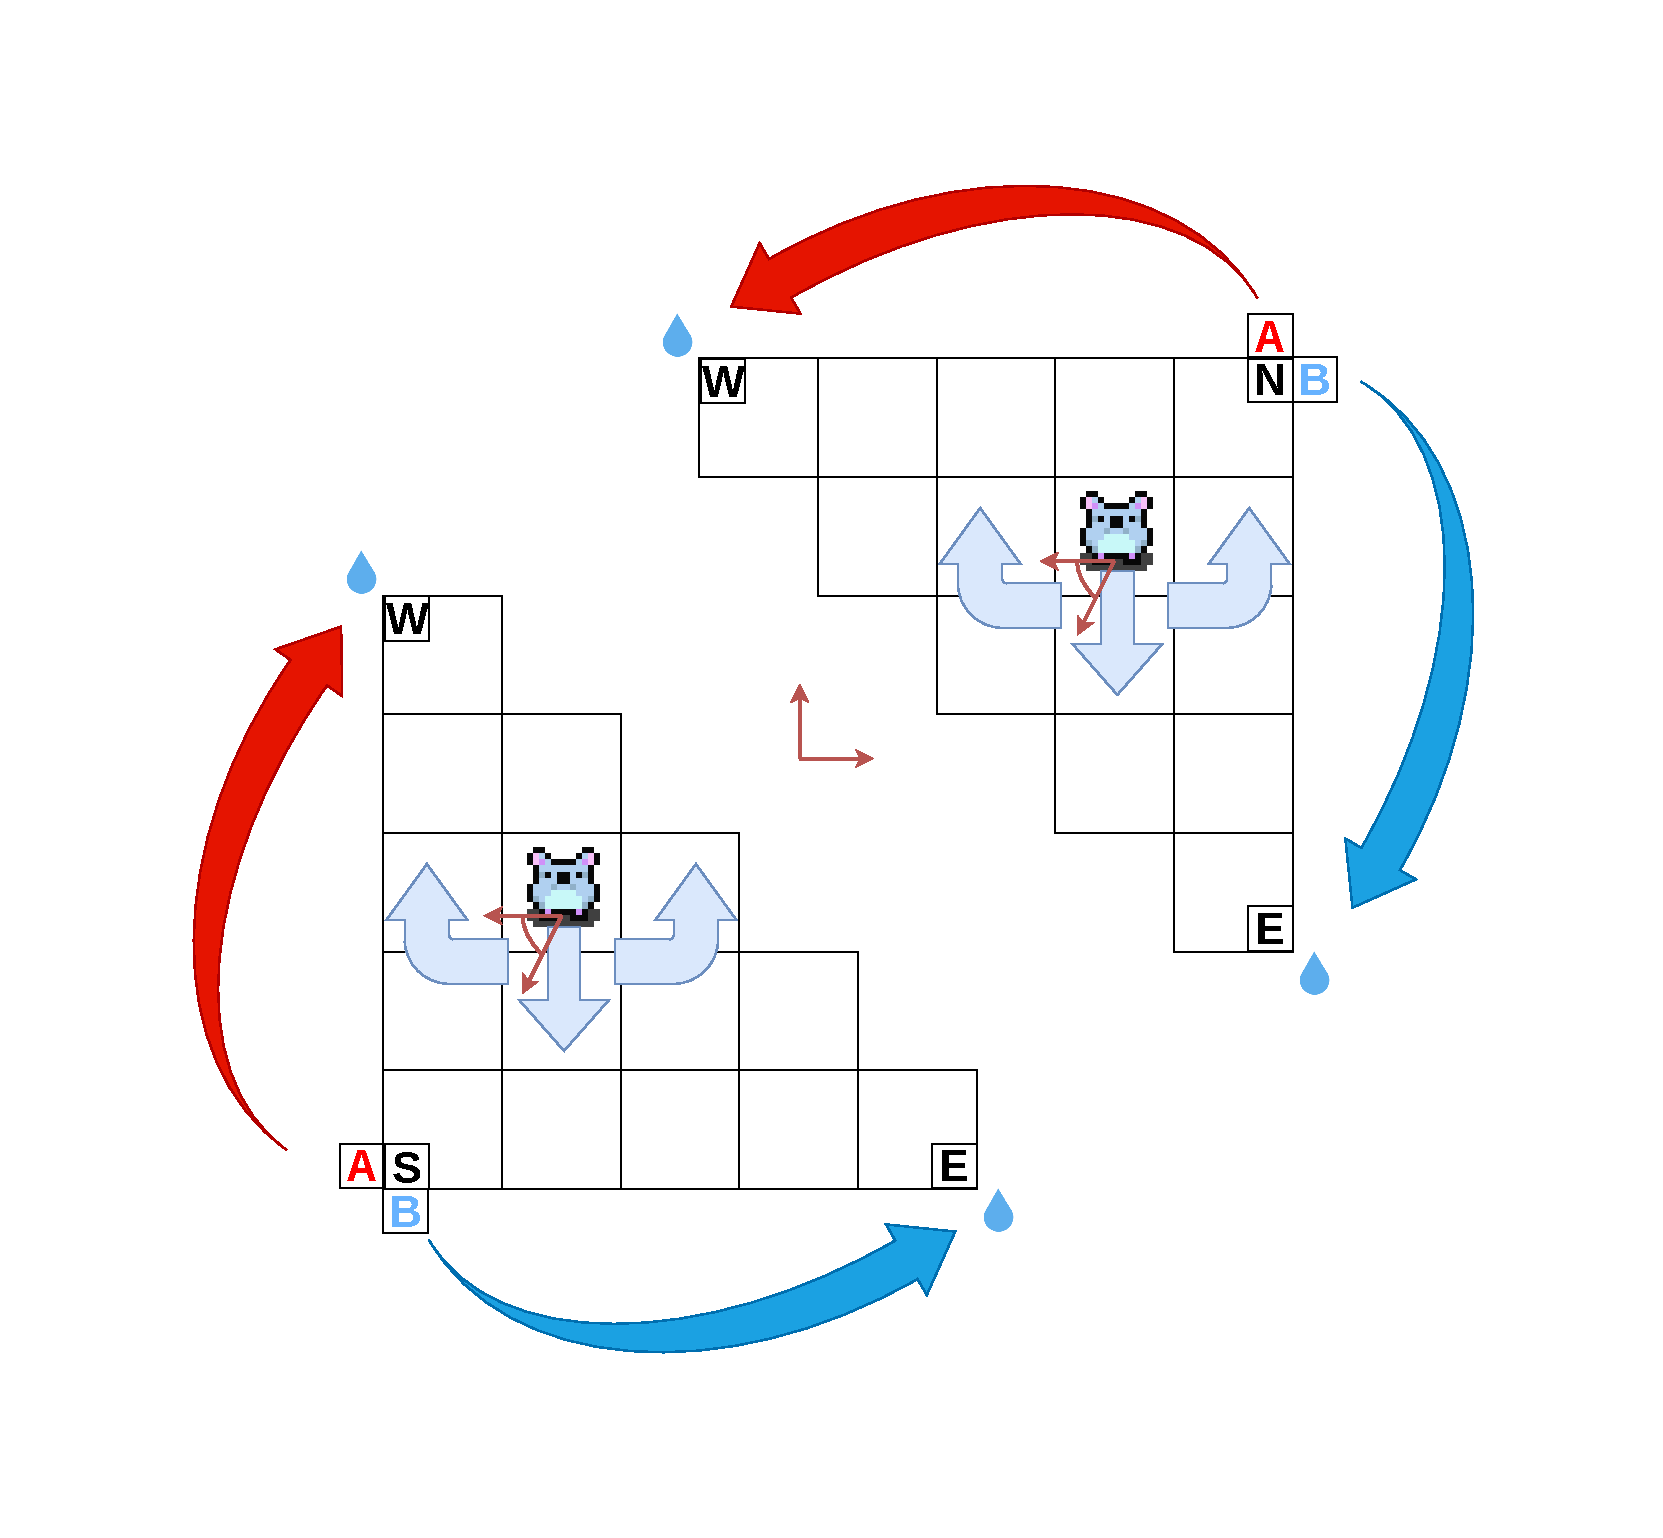
\includegraphics[height=0.55\textheight, trim=3cm 3cm 3cm 3cm, clip=true]{img/RL_env-cartesian-polar.drawio.pdf}
\begin{itemize}
\item Environment: done
\item Training: WIP
\item Visualization: to be improved/discussed
\item Progress are slow as my bandwidth has become very limited
\end{itemize}
\end{frame}
\begin{frame}[label={sec:org0338926}]{State space \& network architecture}
\centering
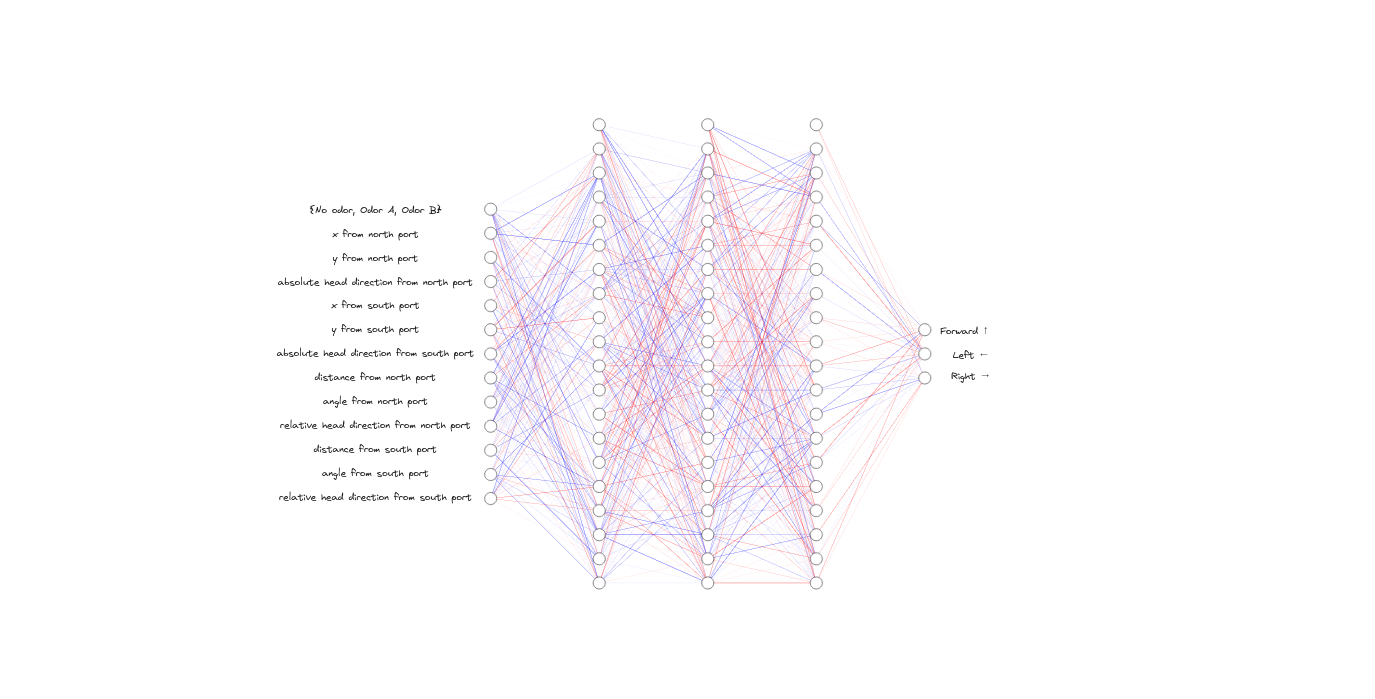
\includegraphics[width=\textwidth, trim=9cm 3cm 10cm 3cm, clip=true]{img/state-space-nn.png}
\tiny
\begin{itemize}
\item 13 inputs + ReLU \(\to\) 512 units  + ReLU \(\to\) 512 units  + ReLU \(\to\) 512 units  + ReLU \(\to\) 3 outputs
\end{itemize}
\end{frame}
\begin{frame}[label={sec:orgf9f5446}]{Training}
\begin{center}
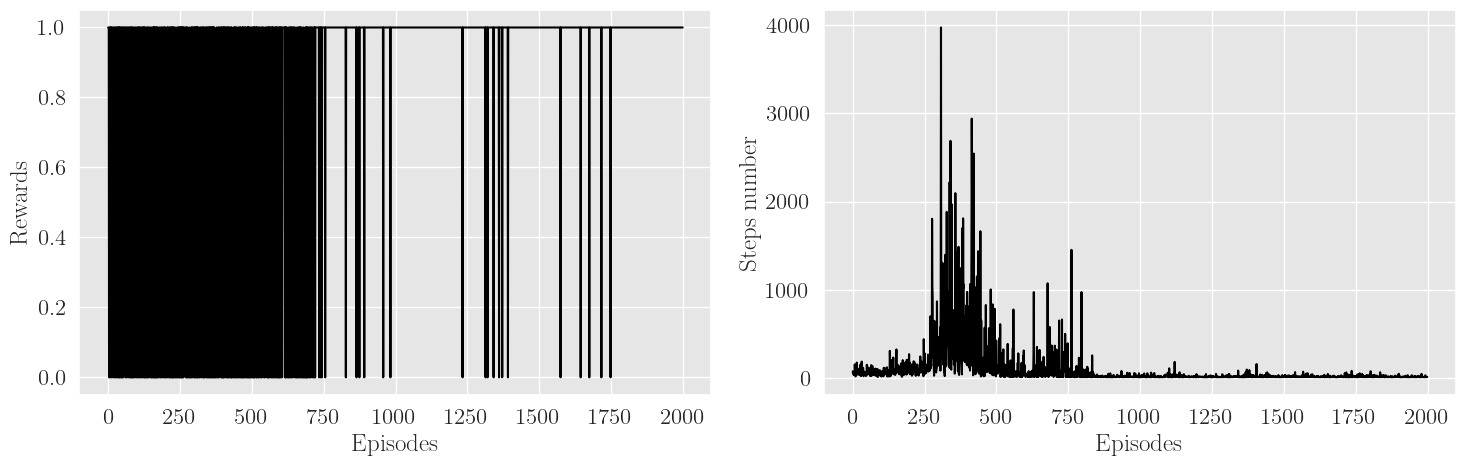
\includegraphics[width=\textwidth]{img/steps-and-rewards.png}
\end{center}
\begin{itemize}
\item 8 hours of training for a single agent on the East/West task
\end{itemize}
\end{frame}
\begin{frame}[label={sec:orgb59c4e4}]{Training checks}
\begin{columns}
\begin{column}[c]{0.5\columnwidth}
\begin{center}
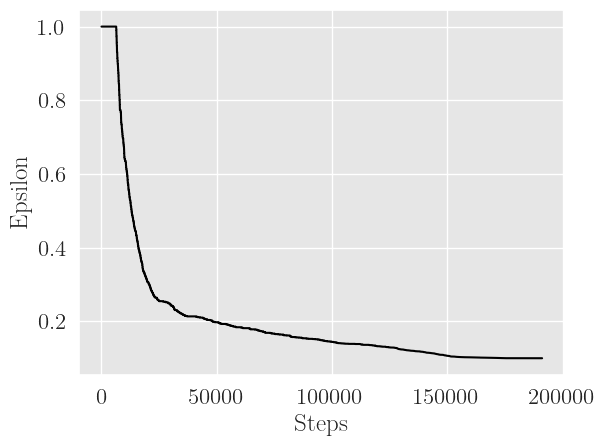
\includegraphics[width=0.8\textwidth]{img/exploration-rate.png}
\end{center}
\begin{center}
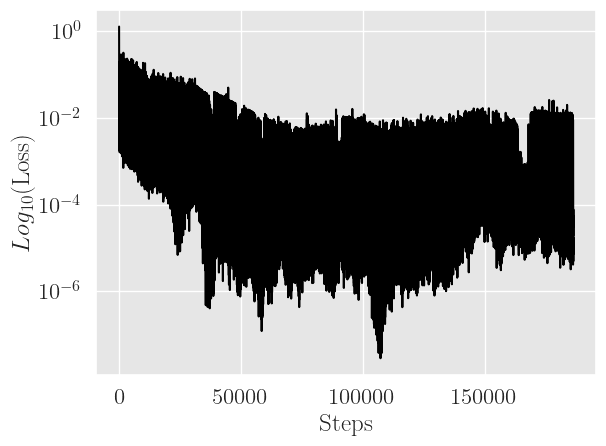
\includegraphics[width=0.8\textwidth]{img/loss.png}
\end{center}
\end{column}
\begin{column}[c]{0.5\columnwidth}
\begin{center}
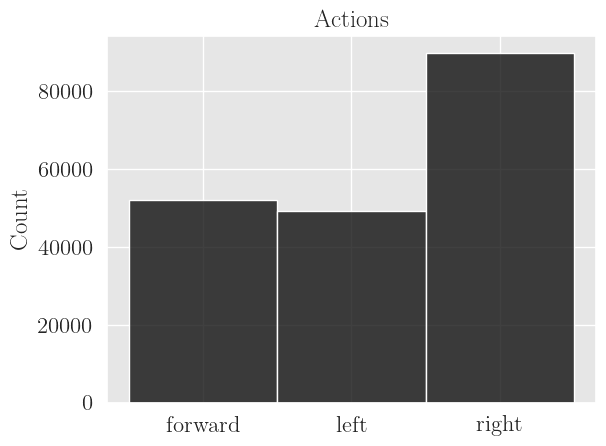
\includegraphics[width=0.65\textwidth]{img/actions-distribution.png}
\end{center}
\begin{center}
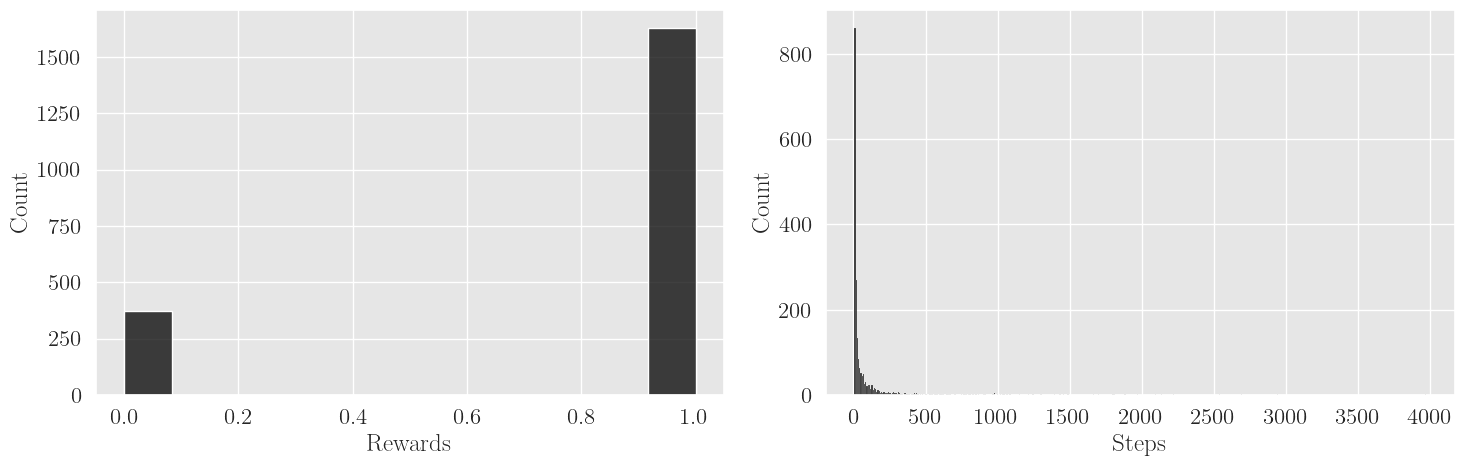
\includegraphics[width=\textwidth]{img/steps-and-rewards-distrib.png}
\end{center}
\end{column}
\end{columns}
\end{frame}
\section{How to visualize the results?}
\label{sec:orgdb0ffba}
\begin{frame}[label={sec:org7c5abed}]{Policy learned}
\begin{center}
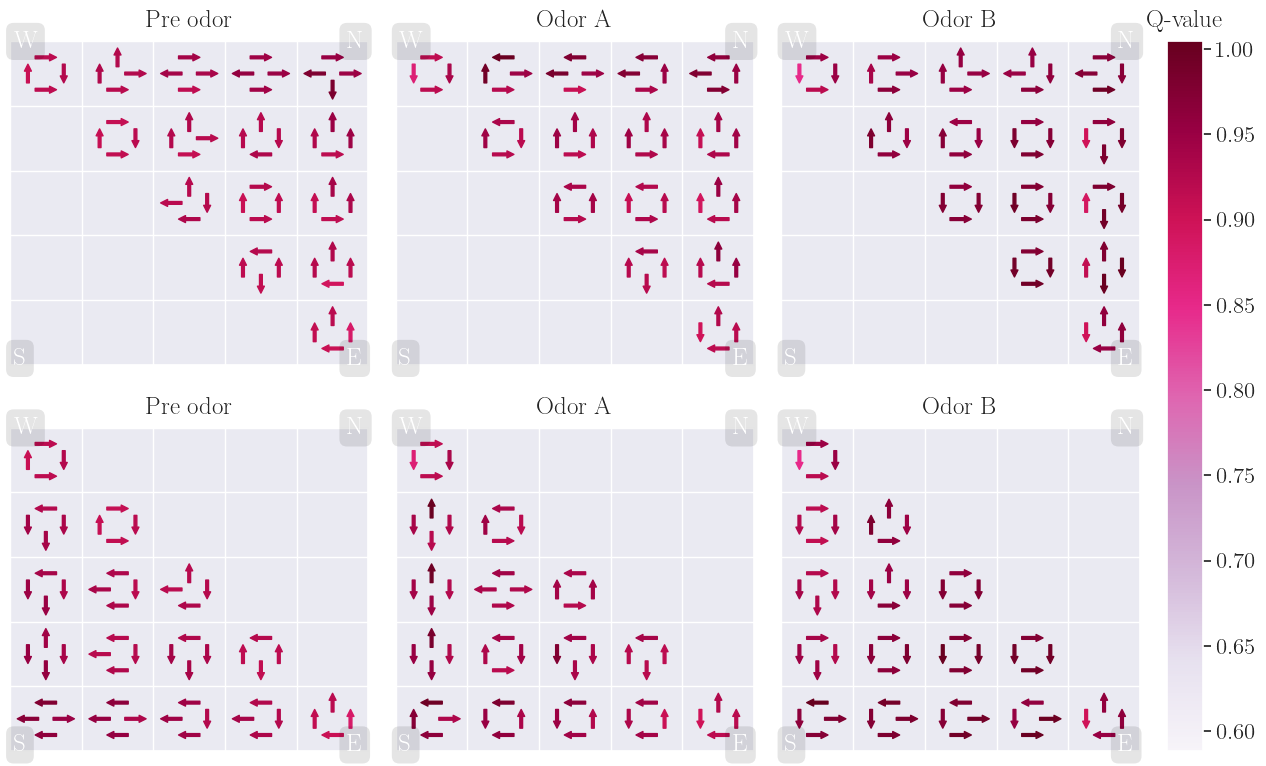
\includegraphics[width=.9\linewidth]{img/policy.png}
\end{center}
\end{frame}
\begin{frame}[label={sec:orga1561a2}]{Weights learned}
\begin{center}
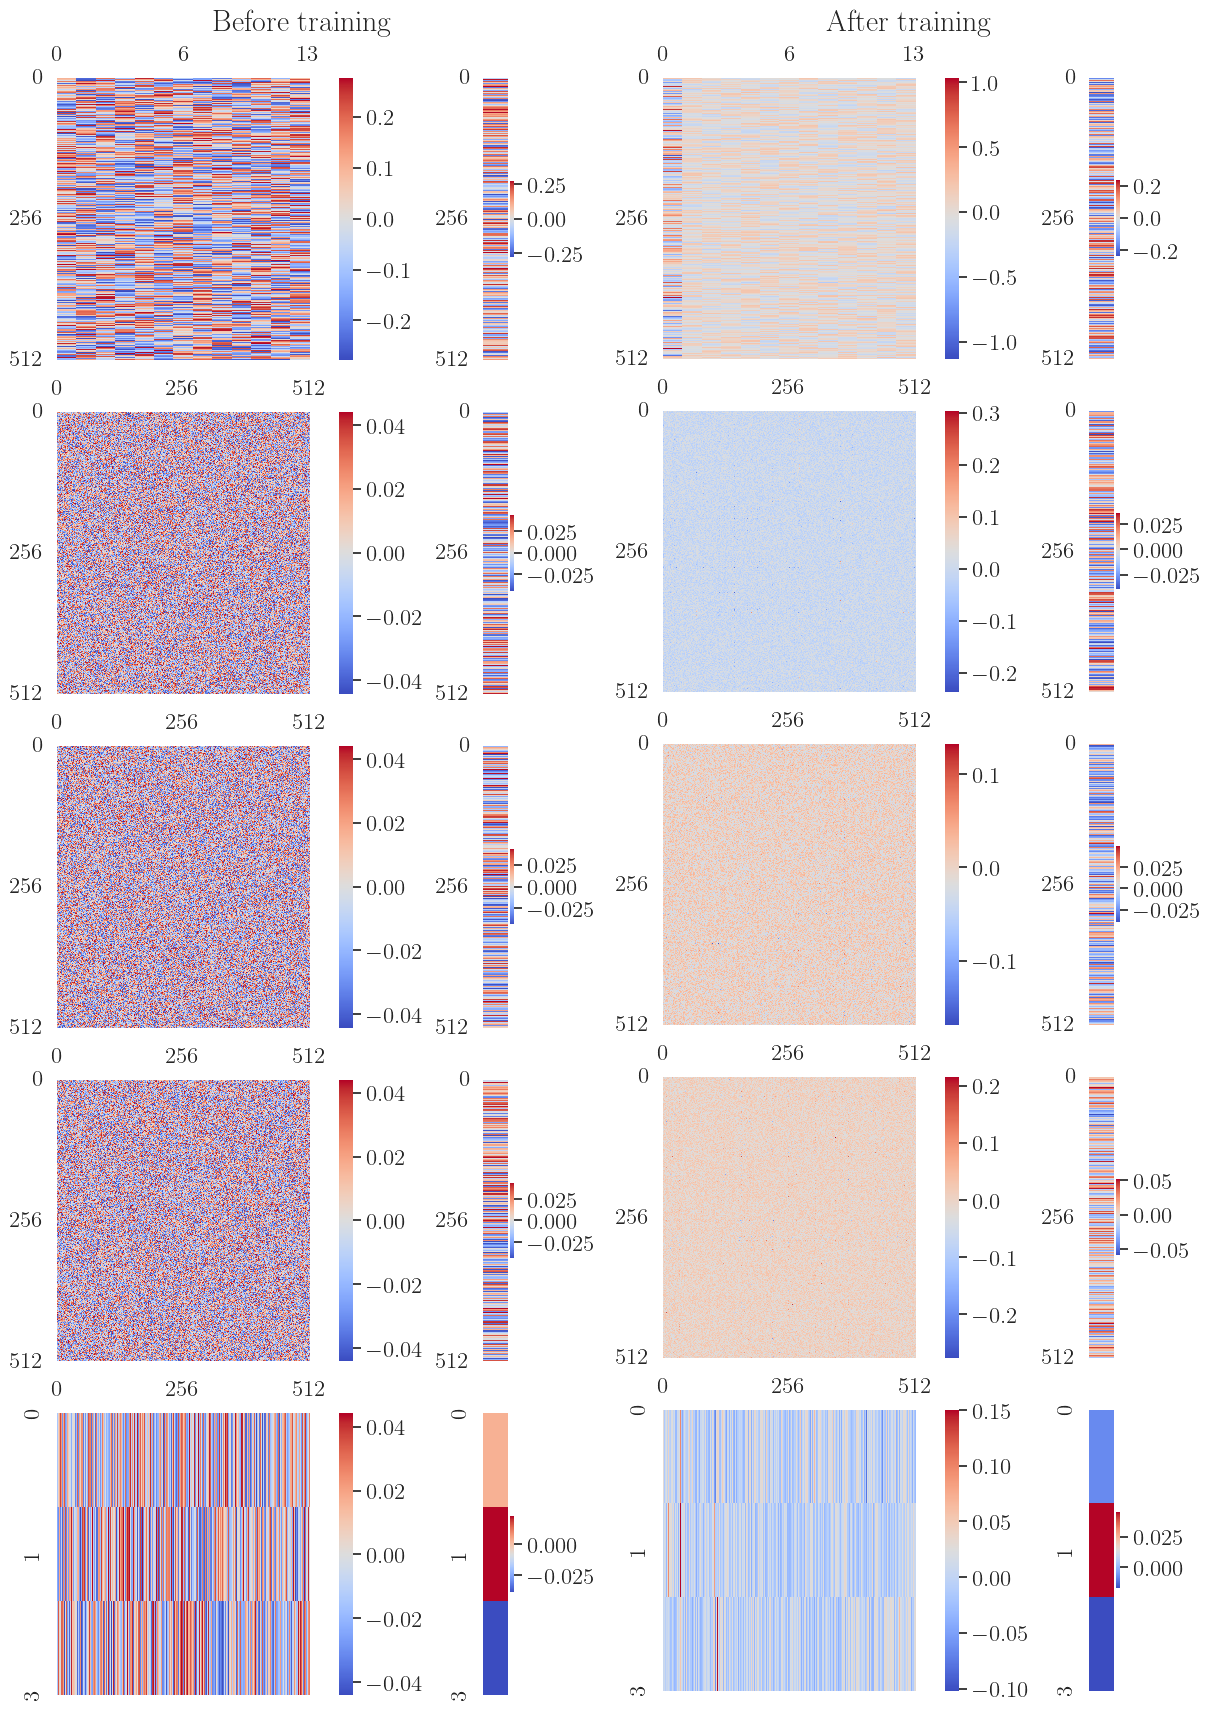
\includegraphics[height=0.9\textheight]{img/weights-matrices.png}
\end{center}
\end{frame}
\begin{frame}[label={sec:org175f551}]{Activations learned}
\begin{center}
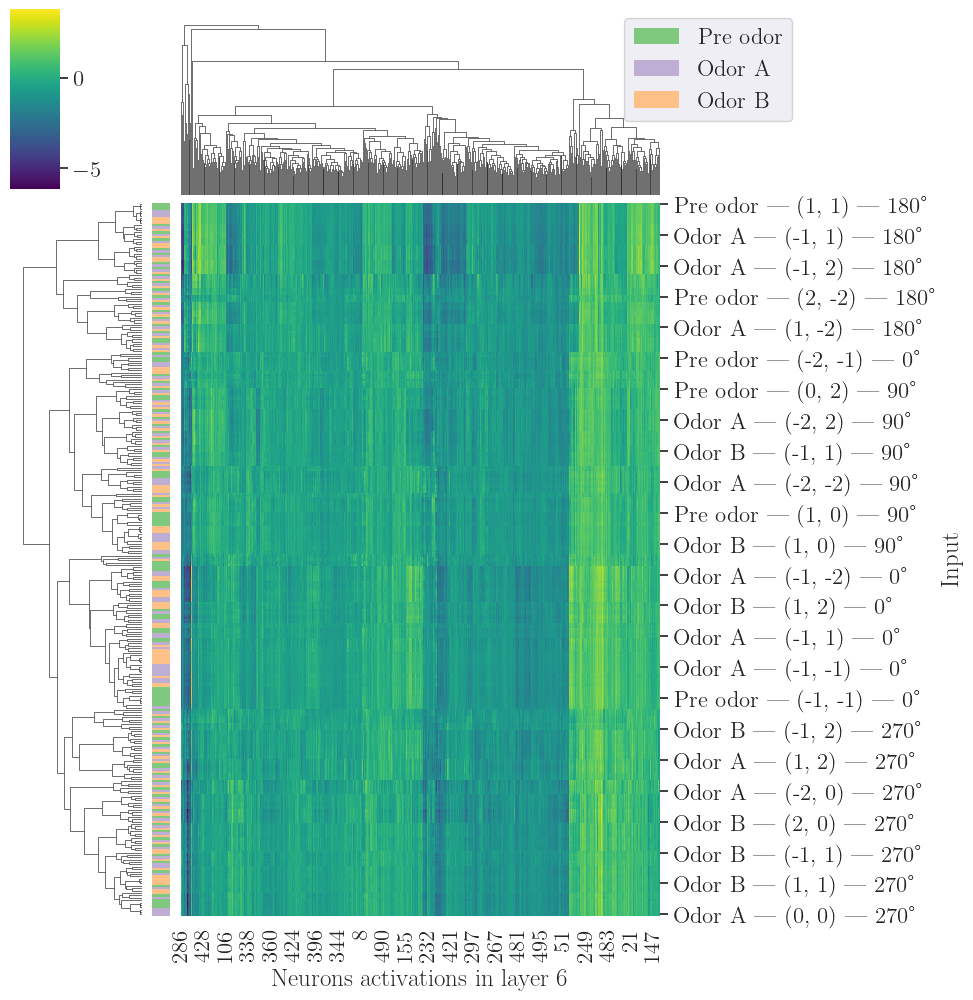
\includegraphics[height=0.9\textheight]{img/activations-learned.png}
\end{center}
\end{frame}
\begin{frame}[label={sec:org5099ea1},standout]{~}
Thanks!
\end{frame}
\end{document}
